\printconcepts

\exercise{In your own words describe what it means for a function to be increasing.}{Answers will vary.}

\exercise{What does a decreasing function ``look like''?}{Answers will vary.}

\exercise{Sketch a graph of a function on $[0,2]$ that is increasing but not strictly increasing.}{Answers will vary.}

\exercise{Give an example of a function describing a situation where it is ``bad'' to be increasing and ``good'' to be decreasing.}{Answers will vary.}

\exercise{A function $f$ has derivative $\fp(x) = (\sin x+2)e^{x^2+1}$, where $\fp(x) >1 $ for all $x$. Is $f$ increasing, decreasing, or can we not tell from the given information?}{Increasing}

\printproblems

\exercise{Given the graph of $f$, identify the intervals of increasing and decreasing as well as the $x$ coordinates of the relative extrema.\\
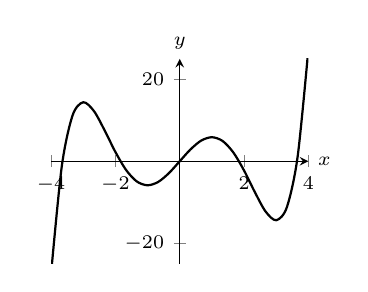
\begin{tikzpicture}
\begin{axis}[width=.4\textwidth,tick label style={font=\scriptsize },
	axis y line=middle,axis x line=middle,
    ymin=-25,ymax=25,
	xmin=-4,xmax=4,name=myplot]
\addplot [{\colorone},smooth,thick,domain=-4:4] {9*x-(10*x*x*x)/3+x*x*x*x*x/5};
\end{axis}
\node [right] at (myplot.right of origin) {\scriptsize $x$};
\node [above] at (myplot.above origin) {\scriptsize $y$};
\end{tikzpicture}}{decreasing on $(-3,-1)$; $(1,3)$,\\
increasing on $(-\infty,-3)$; $(-1,1)$; $(3,\infty)$;\\
local maxima when $x=-3,1$,\\
local minima when $x=-1,3$.}

\exercise{Given the graph of $f$, identify the intervals of increasing and decreasing as well as the $x$ coordinates of the relative extrema.\\
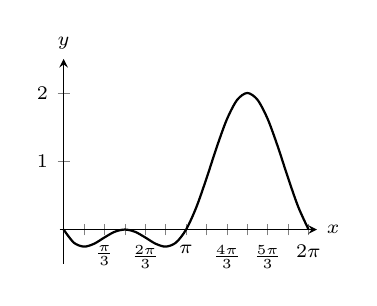
\begin{tikzpicture}
\begin{axis}[width=.4\textwidth,tick label style={font=\scriptsize },
	axis y line=middle,axis x line=middle,
    xtick={0.524,1.047,...,6.5},
	xticklabels={,$\frac\pi3$,,$\frac{2\pi}3$,,$\pi$,,$\frac{4\pi}3$,,$\frac{5\pi}3$,,$2\pi$},
    ymin=-.5,ymax=2.5,
	xmin=-.1,xmax=6.5,name=myplot]
\addplot [{\colorone},smooth,thick,domain=0:6.28] {sin(deg(x))*(sin(deg(x))-1)};
\end{axis}
\node [right] at (myplot.right of origin) {\scriptsize $x$};
\node [above] at (myplot.above origin) {\scriptsize $y$};
\end{tikzpicture}}{decreasing on $(0,\frac\pi6)$; $(\frac\pi2,\frac{5\pi6})$; $(\frac{3\pi}2,2\pi)$,\\
increasing on $(\frac\pi6,\frac\pi2)$; $(\frac{5\pi}6,\frac{3\pi}2)$;\\
local maxima when $x=\frac\pi2,\frac{3\pi}2$,\\
local minima when $x=\frac\pi6,\frac{5\pi}6$.}

%\ifthenelse{\boolean{printquestions}}{\columnbreak}{}

\exercise{Given the graph of $\fp$, identify the intervals of increasing and decreasing as well as the $x$ coordinates of the relative extrema.\\
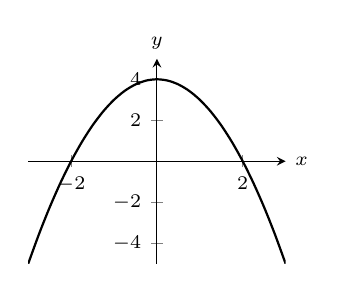
\begin{tikzpicture}
\begin{axis}[width=.4\textwidth,tick label style={font=\scriptsize },
	axis y line=middle,axis x line=middle,
    ymin=-5,ymax=5,
	xmin=-3,xmax=3,name=myplot]
\addplot [{\colorone},smooth,thick,domain=-3:3] {4-x*x};
\end{axis}
\node [right] at (myplot.right of origin) {\scriptsize $x$};
\node [above] at (myplot.above origin) {\scriptsize $y$};
\end{tikzpicture}}{decreasing on $(-\infty,-2)$; $(2,\infty)$,\\
increasing on $(-2,2)$;\\
local maxima when $x=2$,\\
local minima when $x=-2$.}

\exercise{Given the graph of $\fp$, identify the intervals of increasing and decreasing as well as the $x$ coordinates of the relative extrema.\\
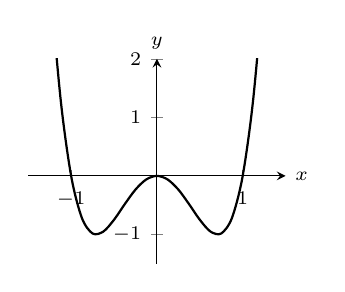
\begin{tikzpicture}
\begin{axis}[width=.4\textwidth,tick label style={font=\scriptsize },
	axis y line=middle,axis x line=middle,
    ymin=-1.5,ymax=2,
	xmin=-1.5,xmax=1.5,name=myplot]
\addplot [{\colorone},smooth,thick,domain=-1.5:1.5] {4*x*x*(x*x-1)};
\end{axis}
\node [right] at (myplot.right of origin) {\scriptsize $x$};
\node [above] at (myplot.above origin) {\scriptsize $y$};
\end{tikzpicture}}{decreasing on $(-1,1)$,\\
increasing on $(-\infty,-1)$; $(1,\infty)$;\\
local maxima when $x=-1$,\\
local minima when $x=1$.}

\exerciseset{In Exercises}{, a function $f(x)$ is given.
	\begin{enumerate}[label=(\alph*)]
	\item	Compute $\fp(x)$.
	\item	Graph $f$ and $\fp$ on the same axes (using technology is permitted) and verify \autoref{thm:incr_decr}.
	\end{enumerate}}{

\exercise{$f(x) = 2x+3$}{Graph and verify.}

\exercise{$f(x) = x^2-3x+5$}{Graph and verify.}

\exercise{$f(x) = \cos x$}{Graph and verify.}

\exercise{$f(x) = \tan x$}{Graph and verify.}

\exercise{$f(x) = x^3-5x^2+7x-1$}{Graph and verify.}

\exercise{$f(x) = 2x^3-x^2+x-1$}{Graph and verify.}

\exercise{$f(x) =x^4-5x^2+4$}{Graph and verify.}

\exercise{$\ds f(x) =\frac{1}{x^2+1}$}{Graph and verify.}

}


%\ifthenelse{\boolean{printquestions}}{\columnbreak}{}

\exerciseset{In Exercises}{, a function $f(x)$ is given.
	\begin{enumerate}
	\item	[(a)] Give the domain of $f$.
	\item	[(b)] Find the critical numbers of $f$.
	\item	[(c)] Create a number line to determine the intervals on which $f$ is increasing and decreasing.
	\item	[(d)] Use the First Derivative Test to determine whether each critical point corresponds to a relative maximum, minimum, or neither.
	\end{enumerate}
}{

\exercise{$\ds f(x) =x^2+2x-3$}{domain: $(-\infty,\infty)$;\\
c.p. at $c=-1$;\\
decreasing on $(-\infty,-1)$;\\
increasing on $(-1,\infty)$;\\
rel. min at $x=-1$.}

\exercise{$\ds f(x) =x^3+3x^2+3$}{domain=$(-\infty,\infty)$;\\
c.p. at $c=-2,0$;\\
increasing on $(-\infty,-2)$; $(0,\infty)$;\\
decreasing on $(-2,0)$;\\
rel. min at $x=0$;\\
rel. max at $x=-2$.}

\exercise{$\ds f(x) =2 x^3+x^2-x+3$}{domain=$(-\infty,\infty)$;\\
c.p. at $c=\frac16(-1\pm\sqrt{7})$;\\
decreasing on $(\frac16(-1-\sqrt{7}),\frac16(-1+\sqrt{7})))$;\\
increasing on $(-\infty,\frac16(-1-\sqrt{7}))$; $(\frac16(-1+\sqrt{7}),\infty)$;\\
rel. min at $x=\frac16(-1+\sqrt{7})$;\\
rel. max at $x=\frac16(-1-\sqrt{7})$.}

\exercise{$\ds f(x) =x^3-3x^2+3x-1$}{domain=$(-\infty,\infty)$\\
c.p. at $c=1$;\\
increasing on $(-\infty,\infty)$}

\exercise{$\ds f(x) =\frac{1}{x^2-2x+2}$}{domain=$(-\infty,\infty)$;\\
c.p. at $c=1$;\\
decreasing on $(1,\infty)$\\
increasing on $(-\infty,1)$;\\
rel. max at $x=1$.}

\exercise{$\ds f(x) =\frac{x^2-4}{x^2-1}$}{domain=$(-\infty,-1)\cup(-1,1)\cup(1,\infty)$;\\
c.p. at $c=0$;\\
decreasing on $(-\infty,-1)$; $(-1,0)$;\\
increasing on $(0,1)$; $(1,\infty)$;\\
rel. min at $x=0$.}

\exercise{$\ds f(x) =\frac{x}{x^2-2x-8}$}{domain=$(-\infty,-2)\cup(-2,4)\cup(4,\infty)$;\\
no c.p.;\\
decreasing on entire domain, $(-\infty,-2)$; $(-2,4)$; $(4,\infty)$.}

\exercise{$\ds f(x) =\frac{(x-2)^{2/3}}{x}$}{domain=$(-\infty,0)\cup(0,\infty)$;\\
c.p. at $c=2,6$;\\
decreasing on $(-\infty,0)$; $(0,2)$; $(6,\infty)$;\\
increasing on $(2,6)$;\\
rel. min at $x=2$;\\
rel. max at $x=6$.}

\exercise{$\ds f(x) =\sin x\cos x$ on $(-\pi,\pi)$.}{domain=$(-\infty,\infty)$;\\
c.p. at $c=-3\pi/4,-\pi/4,\pi/4,3\pi/4$;\\
decreasing on $(-3\pi/4,-\pi/4)$; $(\pi/4,3\pi/4)$;\\
increasing on $(-\pi,-3\pi/4)$; $(-\pi/4,\pi/4)$; $(3\pi/4,\pi)$;\\
rel. min at $x=-\pi/4,3\pi/4$;\\
rel. max at $x=-3\pi/4,\pi/4$.}

\exercise{$\ds f(x) =x^5-5x$}{domain = $(-\infty,\infty)$;\\
c.p. at $c=-1,1$;\\
decreasing on $(-1,1)$;\\
increasing on $(-\infty,-1)$; $(1,\infty)$;\\
rel. min at $x=1$;\\
rel. max at $x=-1$}

\exercise{$\ds f(x) =x-2 \sin x$ on $0\le x\le3\pi$}{domain=$(-\infty,\infty)$;\\
c.p. at $c=\frac\pi3,\frac{5\pi}3,\frac{7\pi}3$;\\
decreasing on $(0,\frac\pi3)$; $(\frac{5\pi}3,\frac{7\pi}3)$;\\
increasing on $(\frac\pi3,\frac{5\pi}3)$; $(\frac{7\pi}3,3\pi)$;\\
rel. min at $x=\frac\pi3,\frac{7\pi}3$;\\
rel. max at $x=\frac{5\pi}3$}

\exercise{$\ds f(x) =\cos^2 x-2 \sin x$ on $0\le x\le2\pi$}{domain=$(-\infty,\infty)$;\\
c.p. at $c=\frac\pi2,\frac{3\pi}2$;\\
decreasing on $(0,\frac\pi2)$; $(\frac{3\pi}2,2\pi)$;\\
increasing on $(\frac\pi2,\frac{3\pi}2)$;\\
rel. min at $x=\frac\pi2$;\\
rel. max at $x=\frac{3\pi}2$}

\exercise{$\ds f(x) =x\sqrt{x-3}$}{domain=$[3,\infty)$;\\
no c.p.;\\
increasing on $(3,\infty)$}

\exercise{$\ds f(x) =(x^2-1)^3$}{domain=$(-\infty,\infty)$;\\
c.p. at $c=-1,0,1$;\\
decreasing on $(-\infty,0)$;\\
increasing on $(0,\infty)$;\\
rel. min at $x=0$}

\exercise{$f(x)=x^{1/3}(x+4)$}{domain=$(-\infty,\infty)$;\\
c.p. at $c=-1,0$;\\
decreasing on $(-\infty,-1)$\\
increasing on $(-1,\infty)$;
rel. min at $x=-1$}

\exercise{$f(\theta)=2\cos\theta+\cos^2\theta$ on $[0,2\pi]$}{domain=$[0,2\pi]$;\\
c.p. at $c=0,\pi, 2\pi$;\\
decreasing on $(0,\pi)$;\\
increasing on $(\pi,2\pi)$;\\
rel. min at $x=\pi$} 

\exercise{$f(x)=2\sqrt x -4x^2$}{domain=$[0,\infty)$;\\
c.p. at $c=1/4$;\\
decreasing on $(1/4,\infty)$;\\
increasing on $(0,1/4)$;
rel. max at $x=1/4$}

\exercise{$f(x)=5x^{2/3}-2x^{5/3}$}{domain=$(-\infty,\infty)$;\\
c.p. at $c=0, 1$;\\
decreasing on $(-\infty,0)$; $(1,\infty)$;\\
increasing on $(0,1$);\\
rel. min at $x=0$;\\
rel. max at $x=1$}

% cut for parity
%\exercise{$f(x)=\frac{1}{2}x^4-4x^2+3$}{domain=$(-\infty,\infty)$;\\
%c.p. at $c=-2,0,2$;\\
%decreasing on $(-\infty,-2)$; $(0,2)$;\\
%increasing on $(-2,0)$; $(2,\infty)$;\\
%rel. max at $x=0$;\\
%rel. min at $x=\pm 2$}

\exercise{$f(x)=\sin^3 x$ on $[0,2\pi]$}{domain=$[0,2\pi]$;\\
c.p. at $c=0,\pi/2,\pi,3\pi/2,2\pi$;\\
decreasing on $(\pi/2, 3\pi/2)$;\\
increasing on $(0,\pi/2)$; $(3\pi/2,2\pi)$;\\
rel. max at $x=\pi/2$;\\
rel. min at $x=3\pi/2$}

\exercise{$f(x)=(x+1)^5-5x-2$}{domain=$(-\infty,\infty)$;\\
c.p. at $c=0,-2$;\\
decreasing on $(-2,0)$;\\
increasing on $(-\infty,-2)$; $(0,\infty)$\\
rel. max at $x=-2$;\\
rel. min at $x=0$}

}


\printreview

\exercise{Consider $f(x) = x^2-3x+5$ on $[-1,2]$; find $c$ guaranteed by the Mean Value Theorem.}{$c=1/2$}

\exercise{Consider $f(x) = \sin x$ on $[-\pi/2,\pi/2]$; find $c$ guaranteed by the Mean Value Theorem.}{$c=\pm \cos^{-1}(2/\pi)$}

